%Experiment
\section{Results}

Under baseline anechoic, noise-free conditions, the method based on an auditory model (1) achieved the highest accuracy, with a Mean Absolute Error (MAE) of $6.59\degree$ ($\pm0.11\degree$). This was followed by the neural network-based method (2) at $8.57\degree$ ($\pm0.19\degree$) and the spatial-spectrogram-based method (3) at $13.54\degree$ ($\pm0.92\degree$). All differences between the methods were statistically significant ($p<0.01$).

Auditory-model-based (1) and neural-network-based methods (2) exhibited varying degrees of noise resilience (Figure~\ref{fig:snr}). The neural-network-based method (2) maintained reasonable performance down to $\mathrm{SNR}=-3\,\mathrm{dB}$, while the~method incorporating an auditory model and decision trees (1) required $\mathrm{SNR}>10\,\mathrm{dB}$ for comparable results. The spatial-spectrogram-based method (3) was the most sensitive to noise, requiring $\mathrm{SNR} \geq 60\,\mathrm{dB}$ to operate reliably. These differences were statistically significant, with $p<0.01$.

\begin{figure}[htbp]
	\begin{center}
		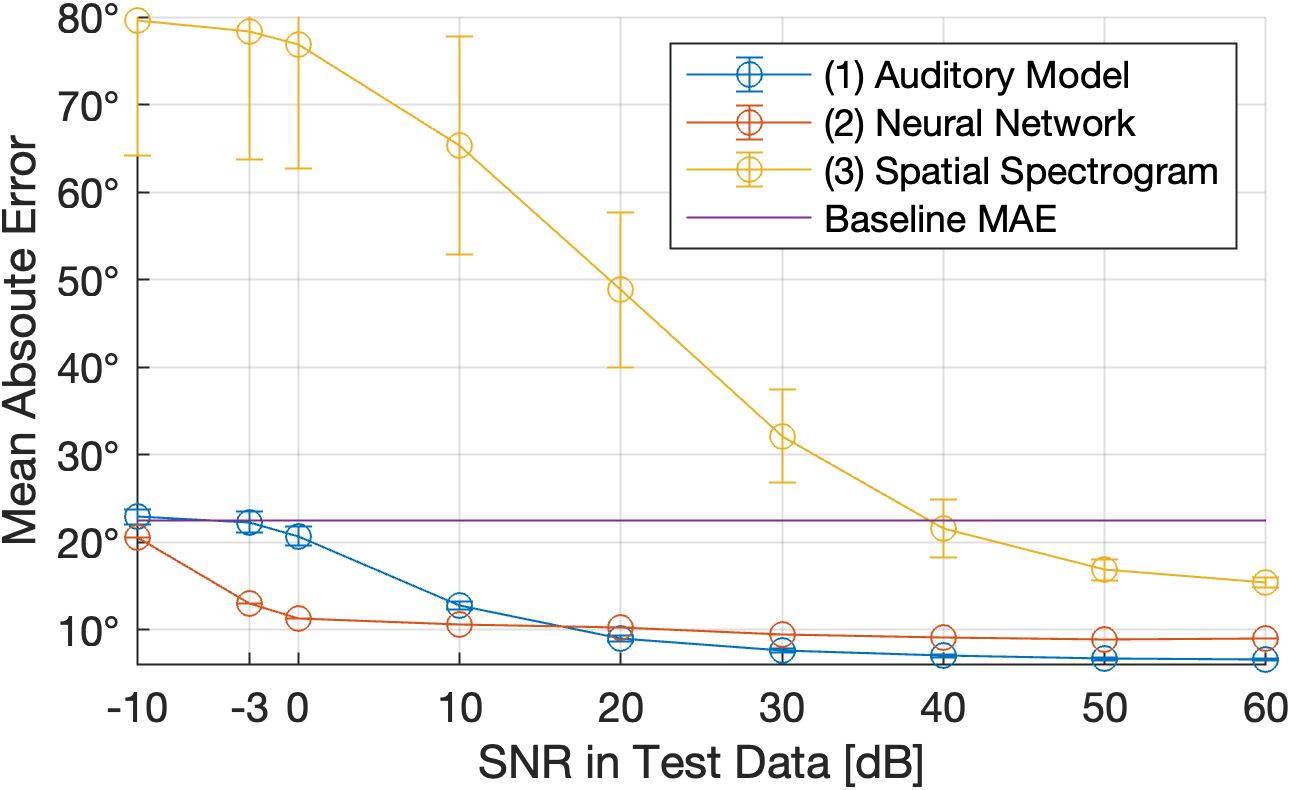
\includegraphics[width=1.0\linewidth]{img/mae_snr_full.png} 
	\end{center}
	\caption{Robustness to noise of the tested methods illustrating the mean absolute error (MAE) at varying signal-to-noise ratios (SNR). Error bars denote standard deviations. The baseline constant predictor (MAE = 22.5°) is included for comparison.} \label{fig:snr}
\end{figure}

Under reverberant conditions, all of the tested methods revealed significant limitations in performance (Figure \ref{fig:rt}). In~particular, the auditory-model-based method demonstrated notable difficulties even at minimal investigated reverberation times ($\mathrm{RT}{60}=0.1\,\mathrm{s}$). While all the methods outperformed the random baseline MAE at $\mathrm{RT}{60}=0.1\,\mathrm{s}$ ($p<0.01$), they demonstrated notable limitations. The primary cause seems to stem from their exclusive training on anechoic signals, leaving them ill-suited for the added temporal and spectral complexity of room reflections.

\begin{figure}[htbp]
	\begin{center}
		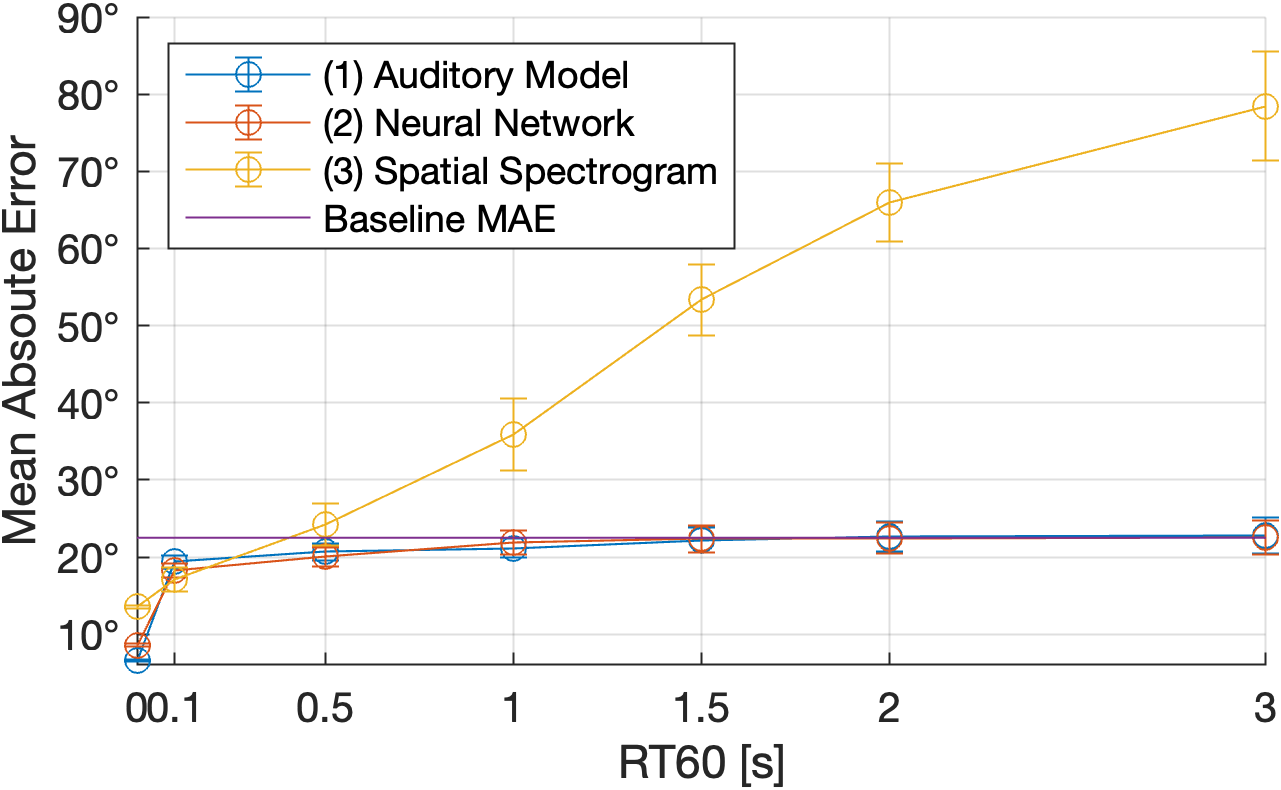
\includegraphics[width=1.0\linewidth]{img/mae_rt.png} 
	\end{center}
	\caption{Robustness to reverberation across tested models, shown as mean absolute error (MAE) for simulated rooms with varying RT60 values. Error bars denote standard deviations. The baseline constant predictor (MAE = 22.5°) is included for comparison.} \label{fig:rt}
\end{figure}

% \begin{figure}[htbp]
% 	\begin{center}
% 		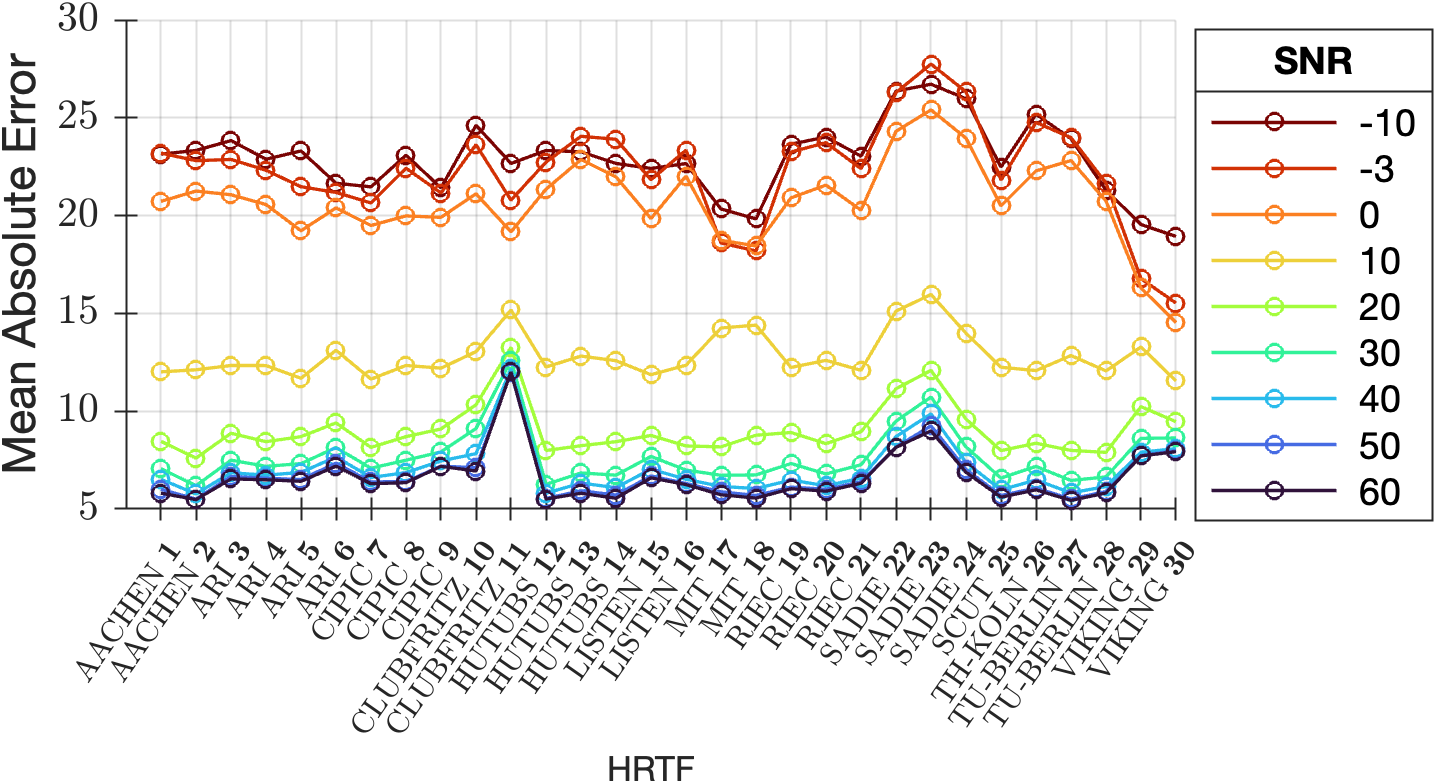
\includegraphics[width=1.0\linewidth]{img/mae_snr_hrtf.png} 
% 	\end{center}
% 	\caption{Mean absolute error (MAE) of ensemble width estimation across different HRTF databases at various signal-to-noise ratios (SNR). The plot demonstrates the varying robustness of the method across different HRTF measurements, with artificial head measurements (marked with *) generally showing more consistent performance compared to human head measurements.} \label{fig:snr_hrtf}
% \end{figure}


% TABLE 
% An example of a floating table. Note that, for IEEE style tables, the
% \caption command should come BEFORE the table. Table text will default to
% \footnotesize as IEEE normally uses this smaller font for tables.
% The \label must come after \caption as always.
%
%\begin{table}[!t]
%% increase table row spacing, adjust to taste
%\renewcommand{\arraystretch}{1.3}
% if using array.sty, it might be a good idea to tweak the value of
% \extrarowheight as needed to properly center the text within the cells
%\caption{An Example of a Table}
%\label{table_example}
%\centering
%% Some packages, such as MDW tools, offer better commands for making tables
%% than the plain LaTeX2e tabular which is used here.
%\begin{tabular}{|c||c|}
%\hline
%One & Two\\
%\hline
%Three & Four\\
%\hline
%\end{tabular}
%\end{table}


% Note that IEEE does not put floats in the very first column - or typically
% anywhere on the first page for that matter. Also, in-text middle ("here")
% positioning is not used. Most IEEE journals use top floats exclusively.
% Note that, LaTeX2e, unlike IEEE journals, places footnotes above bottom
% floats. This can be corrected via the \fnbelowfloat command of the
% stfloats package.


% \begin{table}[ht]
% 		\renewcommand{\arraystretch}{1.3}
% 	\caption{Results of simulation}
% 	\label{results}
% 	\centering
% 	\begin{tabular}{l|c|c|c|c}
% 		\hline\hline
% 		header & abc & ijk & xyz & $\theta$ \\
% 		\hline \hline
% 		one & 0.1 & 0.01 & 0.001 & 0.0001\\ 
% 		\hline
% 		two & 1.1 & 2.2 & 3.3 & 4.4\\
% 		\hline
% 		three & 1.1 & 2.2 & 3.3 & 4.4\\
% 		\hline\hline
% 	\end{tabular}
% \end{table}

% Lorem ipsum dolor sit amet, consectetur adipiscing elit, sed do eiusmod tempor incididunt ut labore et dolore magna aliqua. Ut enim ad minim veniam, quis nostrud exercitation ullamco laboris nisi ut aliquip ex ea commodo consequat. Duis aute irure dolor in reprehenderit in voluptate velit esse cillum dolore eu fugiat nulla pariatur. Excepteur sint occaecat cupidatat non proident, sunt in culpa qui officia deserunt mollit anim id est laborum.

% \subsection{Subsection Heading Here}
% Lorem ipsum dolor sit amet, consectetur adipiscing elit, sed do eiusmod tempor incididunt ut labore et dolore magna aliqua. Ut enim ad minim veniam, quis nostrud exercitation ullamco laboris nisi ut aliquip ex ea commodo consequat. Duis aute irure dolor in reprehenderit in voluptate velit esse cillum dolore eu fugiat nulla pariatur. Excepteur sint occaecat cupidatat non proident, sunt in culpa qui officia deserunt mollit anim id est laborum.

% % needed in second column of first page if using \IEEEpubid
% %\IEEEpubidadjcol

% \subsubsection{Subsubsection Heading Here}

% Lorem ipsum dolor sit amet, consectetur adipiscing elit, sed do eiusmod tempor incididunt ut labore et dolore magna aliqua. Ut enim ad minim veniam, quis nostrud exercitation ullamco laboris nisi ut aliquip ex ea commodo consequat (\ref{eq:2}).

% \begin{equation} \label{eq:2}
% 	\frac{{dP}}{{dt}} \approx \frac{{P_{k + 1}  - P_k }}{T}
% \end{equation}

% \subsubsection{Subsubsection Heading Here}

%  Duis aute irure dolor in reprehenderit in voluptate velit esse cillum dolore eu fugiat nulla pariatur. Excepteur sint occaecat cupidatat non proident, sunt in culpa qui officia deserunt mollit anim id est laborum.

% Lorem ipsum dolor sit amet, consectetur adipiscing elit, sed do eiusmod tempor incididunt ut labore et dolore magna aliqua. Ut enim ad minim veniam, quis nostrud exercitation ullamco laboris nisi ut aliquip ex ea commodo consequat. Duis aute irure dolor in reprehenderit in voluptate velit esse cillum dolore eu fugiat nulla pariatur. Excepteur sint occaecat cupidatat non proident, sunt in culpa qui officia deserunt mollit anim id est laborum.

% \subsection{Subsection Heading Here}
% Lorem ipsum dolor sit amet, consectetur adipiscing elit, sed do eiusmod tempor incididunt ut labore et dolore magna aliqua. Ut enim ad minim veniam, quis nostrud exercitation ullamco laboris nisi ut aliquip ex ea commodo consequat. Duis aute irure dolor in reprehenderit in voluptate velit esse cillum dolore eu fugiat nulla pariatur. Excepteur sint occaecat cupidatat non proident, sunt in culpa qui officia deserunt mollit anim id est laborum. Simulation times for each presented scenario are shown in Table~\ref{table_two}.

% \begin{table}[h]
% 	% increase table row spacing, adjust to taste
% 	\renewcommand{\arraystretch}{1.3}
% 	% if using array.sty, it might be a good idea to tweak the value of \\extrarowheight as needed to properly center the text within the cells
% 	\caption{Simulation times of each scenario}
% 	\label{table_two}
% 	\centering
% 	\begin{tabular}{l|c|c|c}
% 		\hline\hline
% 		& White~[s] & Black~[s] & White to Black\\
% 		\hline\hline
% 		scenario 1 & 5 & 15 & 3 x faster\\
% 		\hline
% 		scenario 2 & 3 & 21 & 7 x faster\\
% 		\hline
% 		scenario 3 & 4 & 24 & 6 x faster\\
% 		\hline
% 		scenario 4 & 7 & 56 & 8 x faster\\
% 		\hline
% 		scenario 5 & 10 & 120 & 12 x faster\\
% 		\hline
% 		scenario 6 & 12 & 24 & 2 x faster\\
% 		\hline\hline
% 	\end{tabular}
% \end{table}

% Lorem ipsum dolor sit amet, consectetur adipiscing elit, sed do eiusmod tempor incididunt ut labore et dolore magna aliqua. Ut enim ad minim veniam, quis nostrud exercitation ullamco laboris nisi ut aliquip ex ea commodo consequat. Duis aute irure dolor in reprehenderit in voluptate velit esse cillum dolore eu fugiat nulla pariatur. Excepteur sint occaecat cupidatat non proident, sunt in culpa qui officia deserunt mollit anim id est laborum.









